% =====================================================================
% 2  Original meta-analysis and replication
%                                      Folien 6-8 | 4:00 min | bis 8:45
% Inhalt: Bericht Kap. 3-4. Backup A1 (alle Schaetzer) ist verlinkt.
% =====================================================================
\section{Original meta-analysis and replication}

% ---------------------------------------------------------------------
\begin{frame}{The original meta-analysis: \citet{zschirnt2016}}
  \timing{1:15}{6:00}
  \begin{itemize}
    \item \todo{Selection: correspondence tests in OECD countries,
      testing years 1990--2015, written applications only}
    \item \todo{Sample: 43 studies; \maK{} studies (\maKsub{} subgroups)
      report call-back counts and enter the pooled odds ratio}
    \item \todo{Method: random effects (REML), one estimate per study}
    \item \todo{Main result: OR \maORre{} \maCIre}
  \end{itemize}
  \keymsg{\todo{Key message of this slide in one sentence}}
\end{frame}

% ---------------------------------------------------------------------
\begin{frame}[label=replication]{Replication of the pooled effect ($k = \maK$)}
  \timing{1:30}{7:30}
  \centering
  \begin{tabular}{lccc}
    \toprule
    Model & OR [95\% CI] & $\hat\tau^2$ & $I^2$ (\%) \\
    \midrule
    Fixed effect (FE)     & \maORfe{} \maCIfe     & -- & -- \\
    UWLS                  & \maORuwls{} \maCIuwls & -- & -- \\
    Random effects (REML) & \maORre{} \maCIre     & \maTauSqRe & \maIsqRe \\
    \midrule
    \citet{zschirnt2016}, RE (REML) & 0.60 [0.52; 0.69] & 0.141 & 92.7 \\
    \bottomrule
  \end{tabular}

  \raggedright
  \begin{itemize}
    \item \todo{Replication is exact}
    \item \todo{Same point estimate for FE and UWLS, but UWLS SE is
      \maSEratioUWLS{} times larger $\Rightarrow$ heterogeneity}
  \end{itemize}
  \keymsg{\todo{Key message of this slide in one sentence}}
  \buttons{\gotobackup{app-replication}{All estimators}}
\end{frame}

% ---------------------------------------------------------------------
\begin{frame}{Forest plot: original studies}
  \timing{1:15}{8:45}
  \begin{columns}[T]
    \begin{column}{0.56\textwidth}
      \centering
      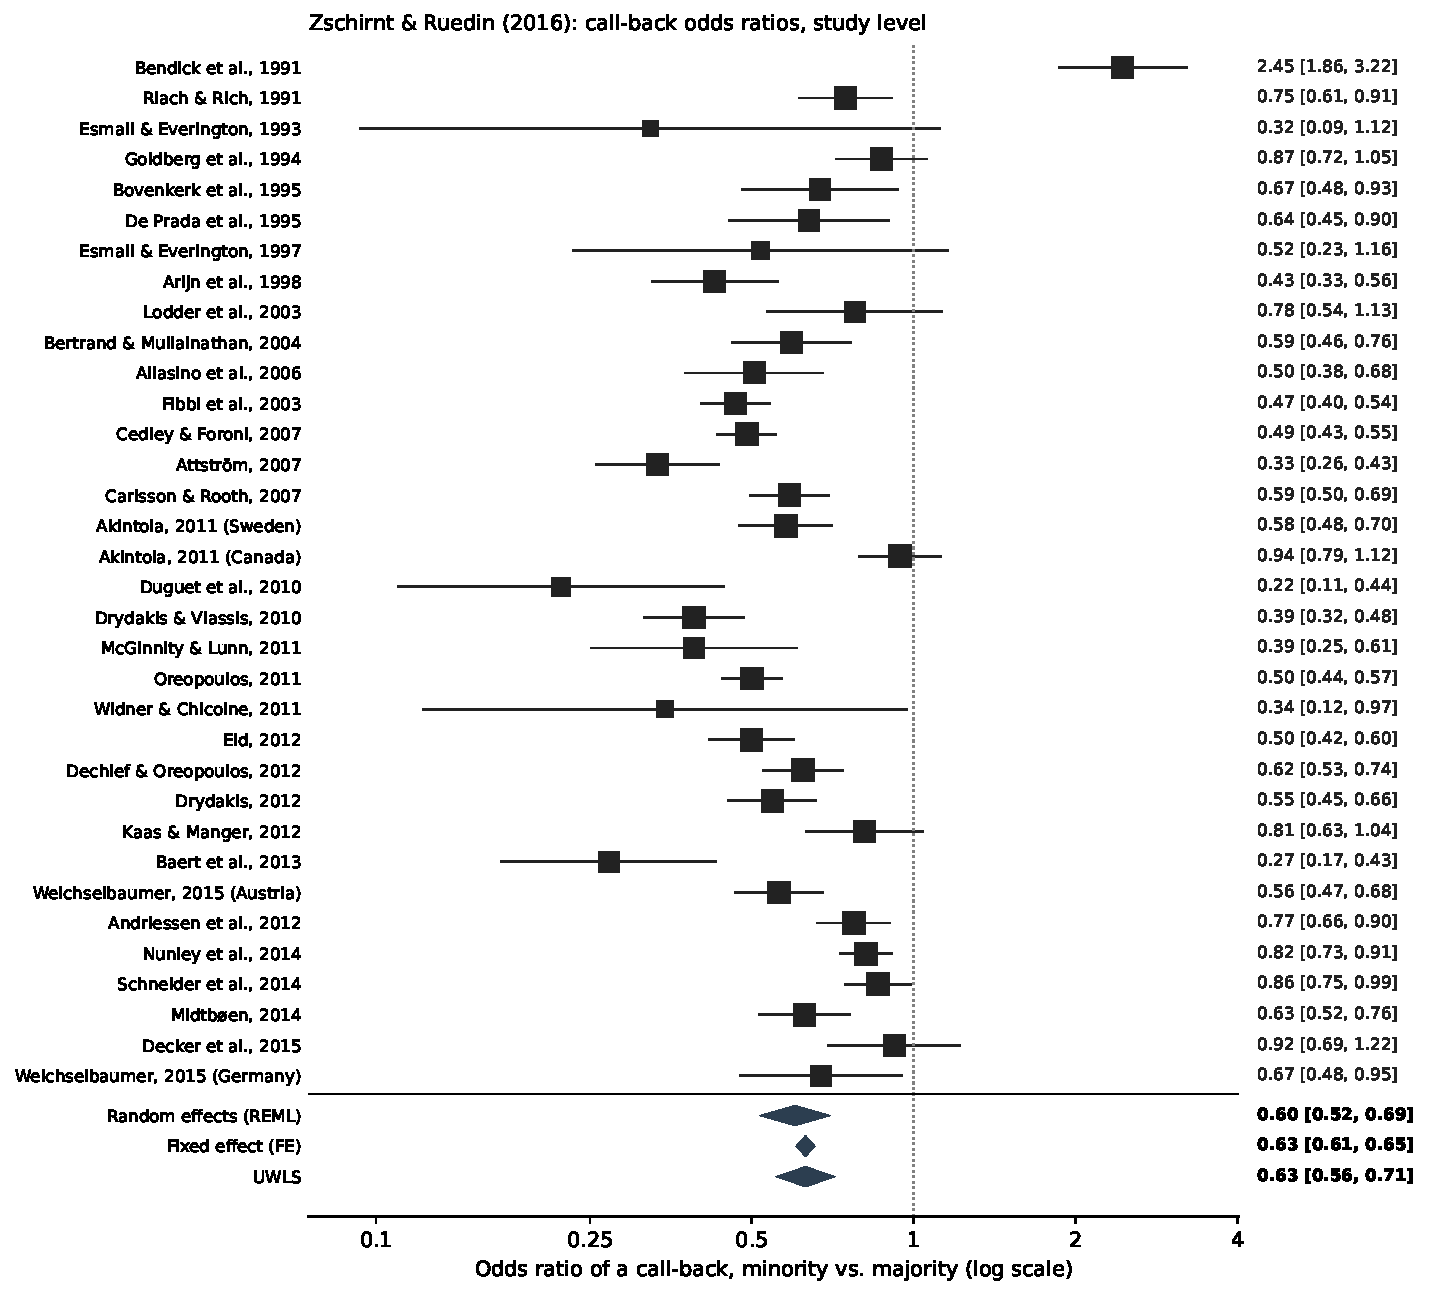
\includegraphics[height=0.82\textheight]{forest_original}
    \end{column}
    \begin{column}{0.42\textwidth}
      \begin{itemize}
        \item \todo{What the plot shows: direction, spread, outliers}
        \item \todo{Heterogeneity: $I^2 = \maIsqRe\,\%$; prediction
          interval \maPIre{} includes 1}
        \item \todo{Outlier Bendick et al.\ (1991): kept in the main
          model, as in the original}
      \end{itemize}
      \medskip
      \todo{Key message}
    \end{column}
  \end{columns}
\end{frame}
